\section{Introduction to nonlinear Schwarz methods}
\begin{frame}{Nonlinear domain decomposition methods}
	Discretized nonlinear partial differential equation: $F(u) = 0$
	\begin{block}{\normalsize Classical approach}
		\begin{tikzpicture}[node distance=7cm]
			% \node[inner sep=0pt] (one) at (-5,1.5){\Large\emph{\underline{Classical approach}}};
			\node[inner sep=0pt] (one) at (-5,0)
			{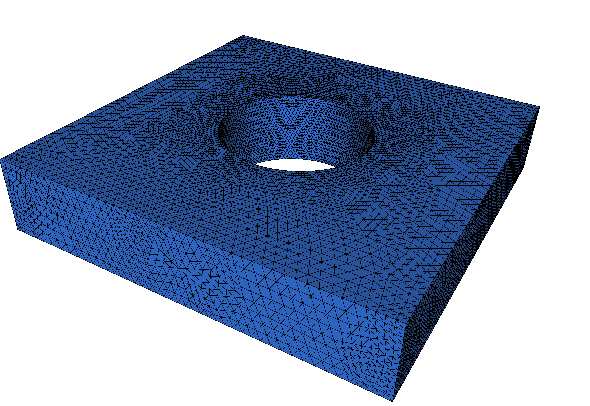
\includegraphics[width=2.9cm]{images/eps/rechteckring58534p_64001.pdf}};

			\node[inner sep=0pt] (two) at (-1,0)
			{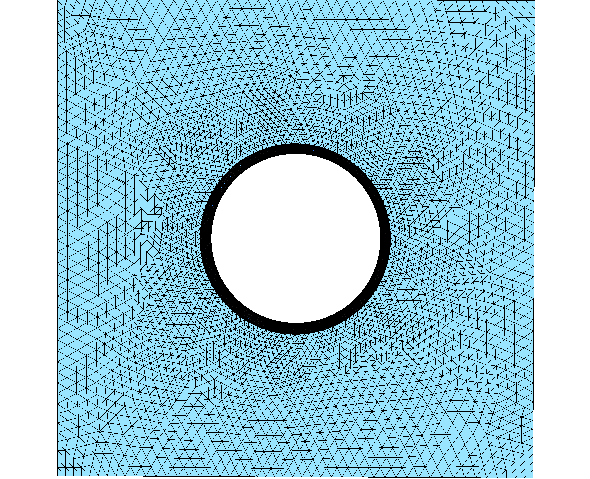
\includegraphics[width=2.2cm]{images/eps/rechteckring58534p_copy008.pdf}};
			\node[inner sep=0pt] (three) at (2.7,0)
			{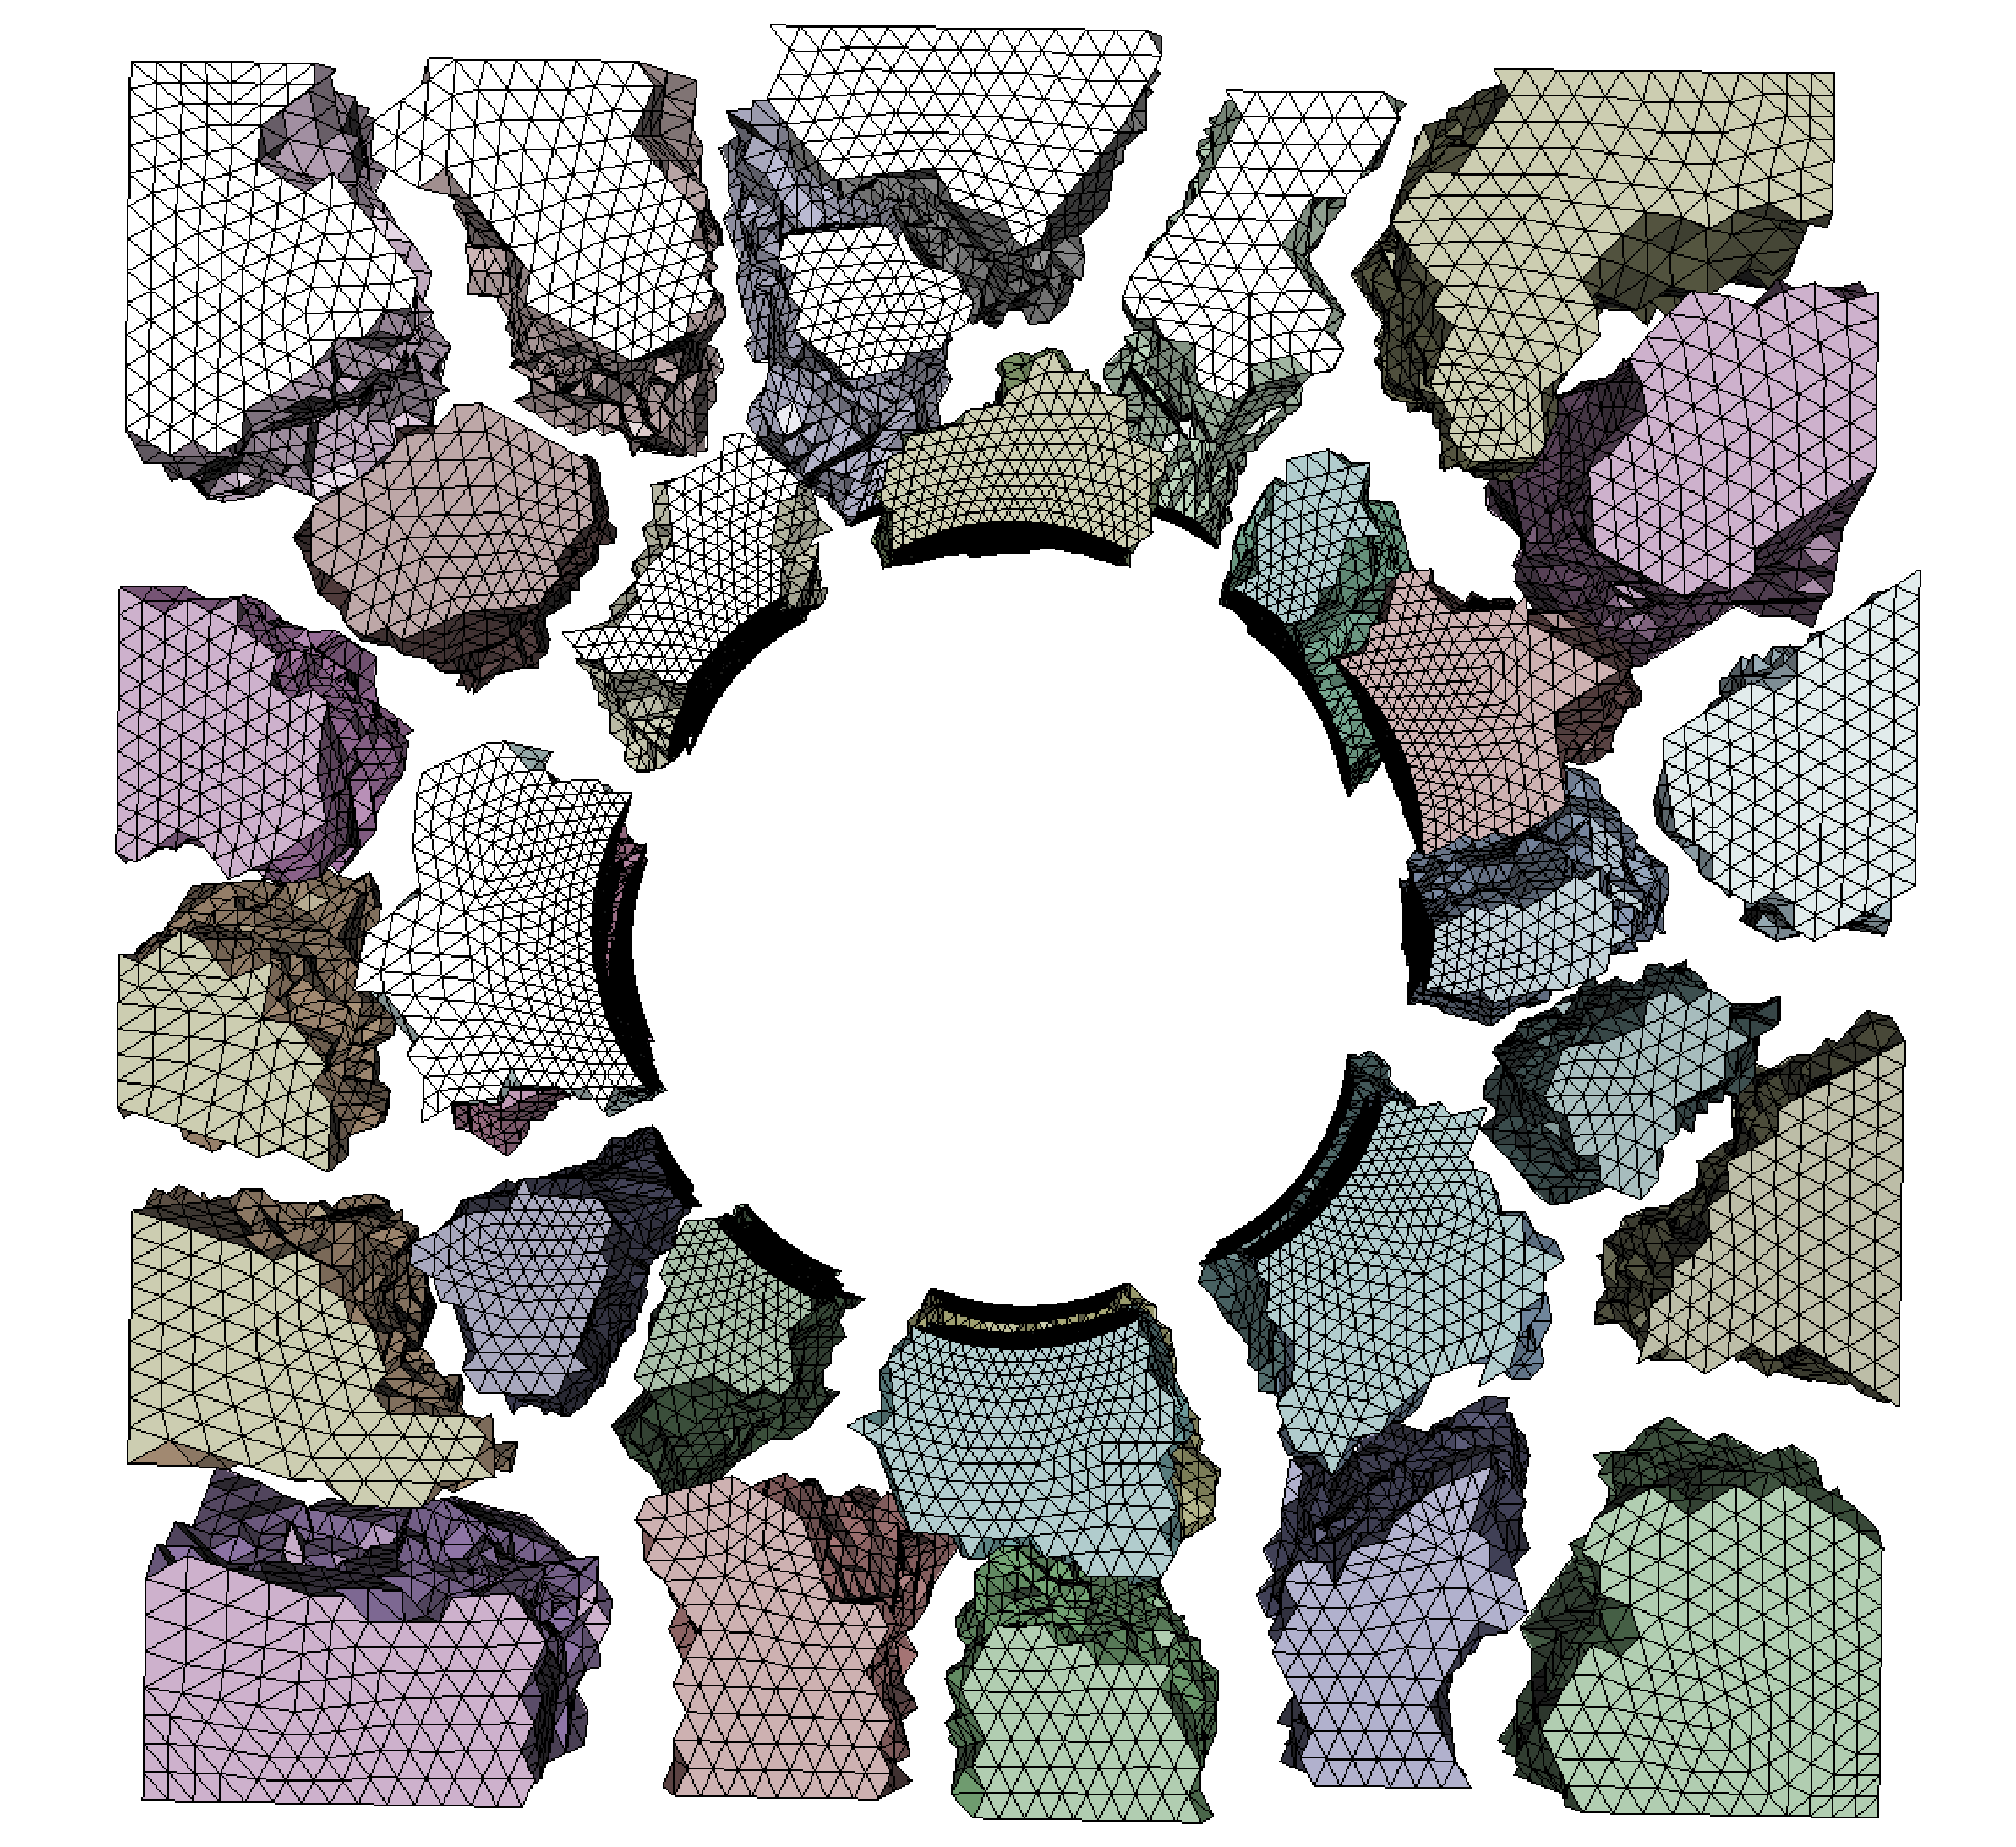
\includegraphics[width=2.0cm]{images/eps/exploded_5004_entsaettigt3.pdf}};
			\node[inner sep=0pt] (four) at (6,0)
			{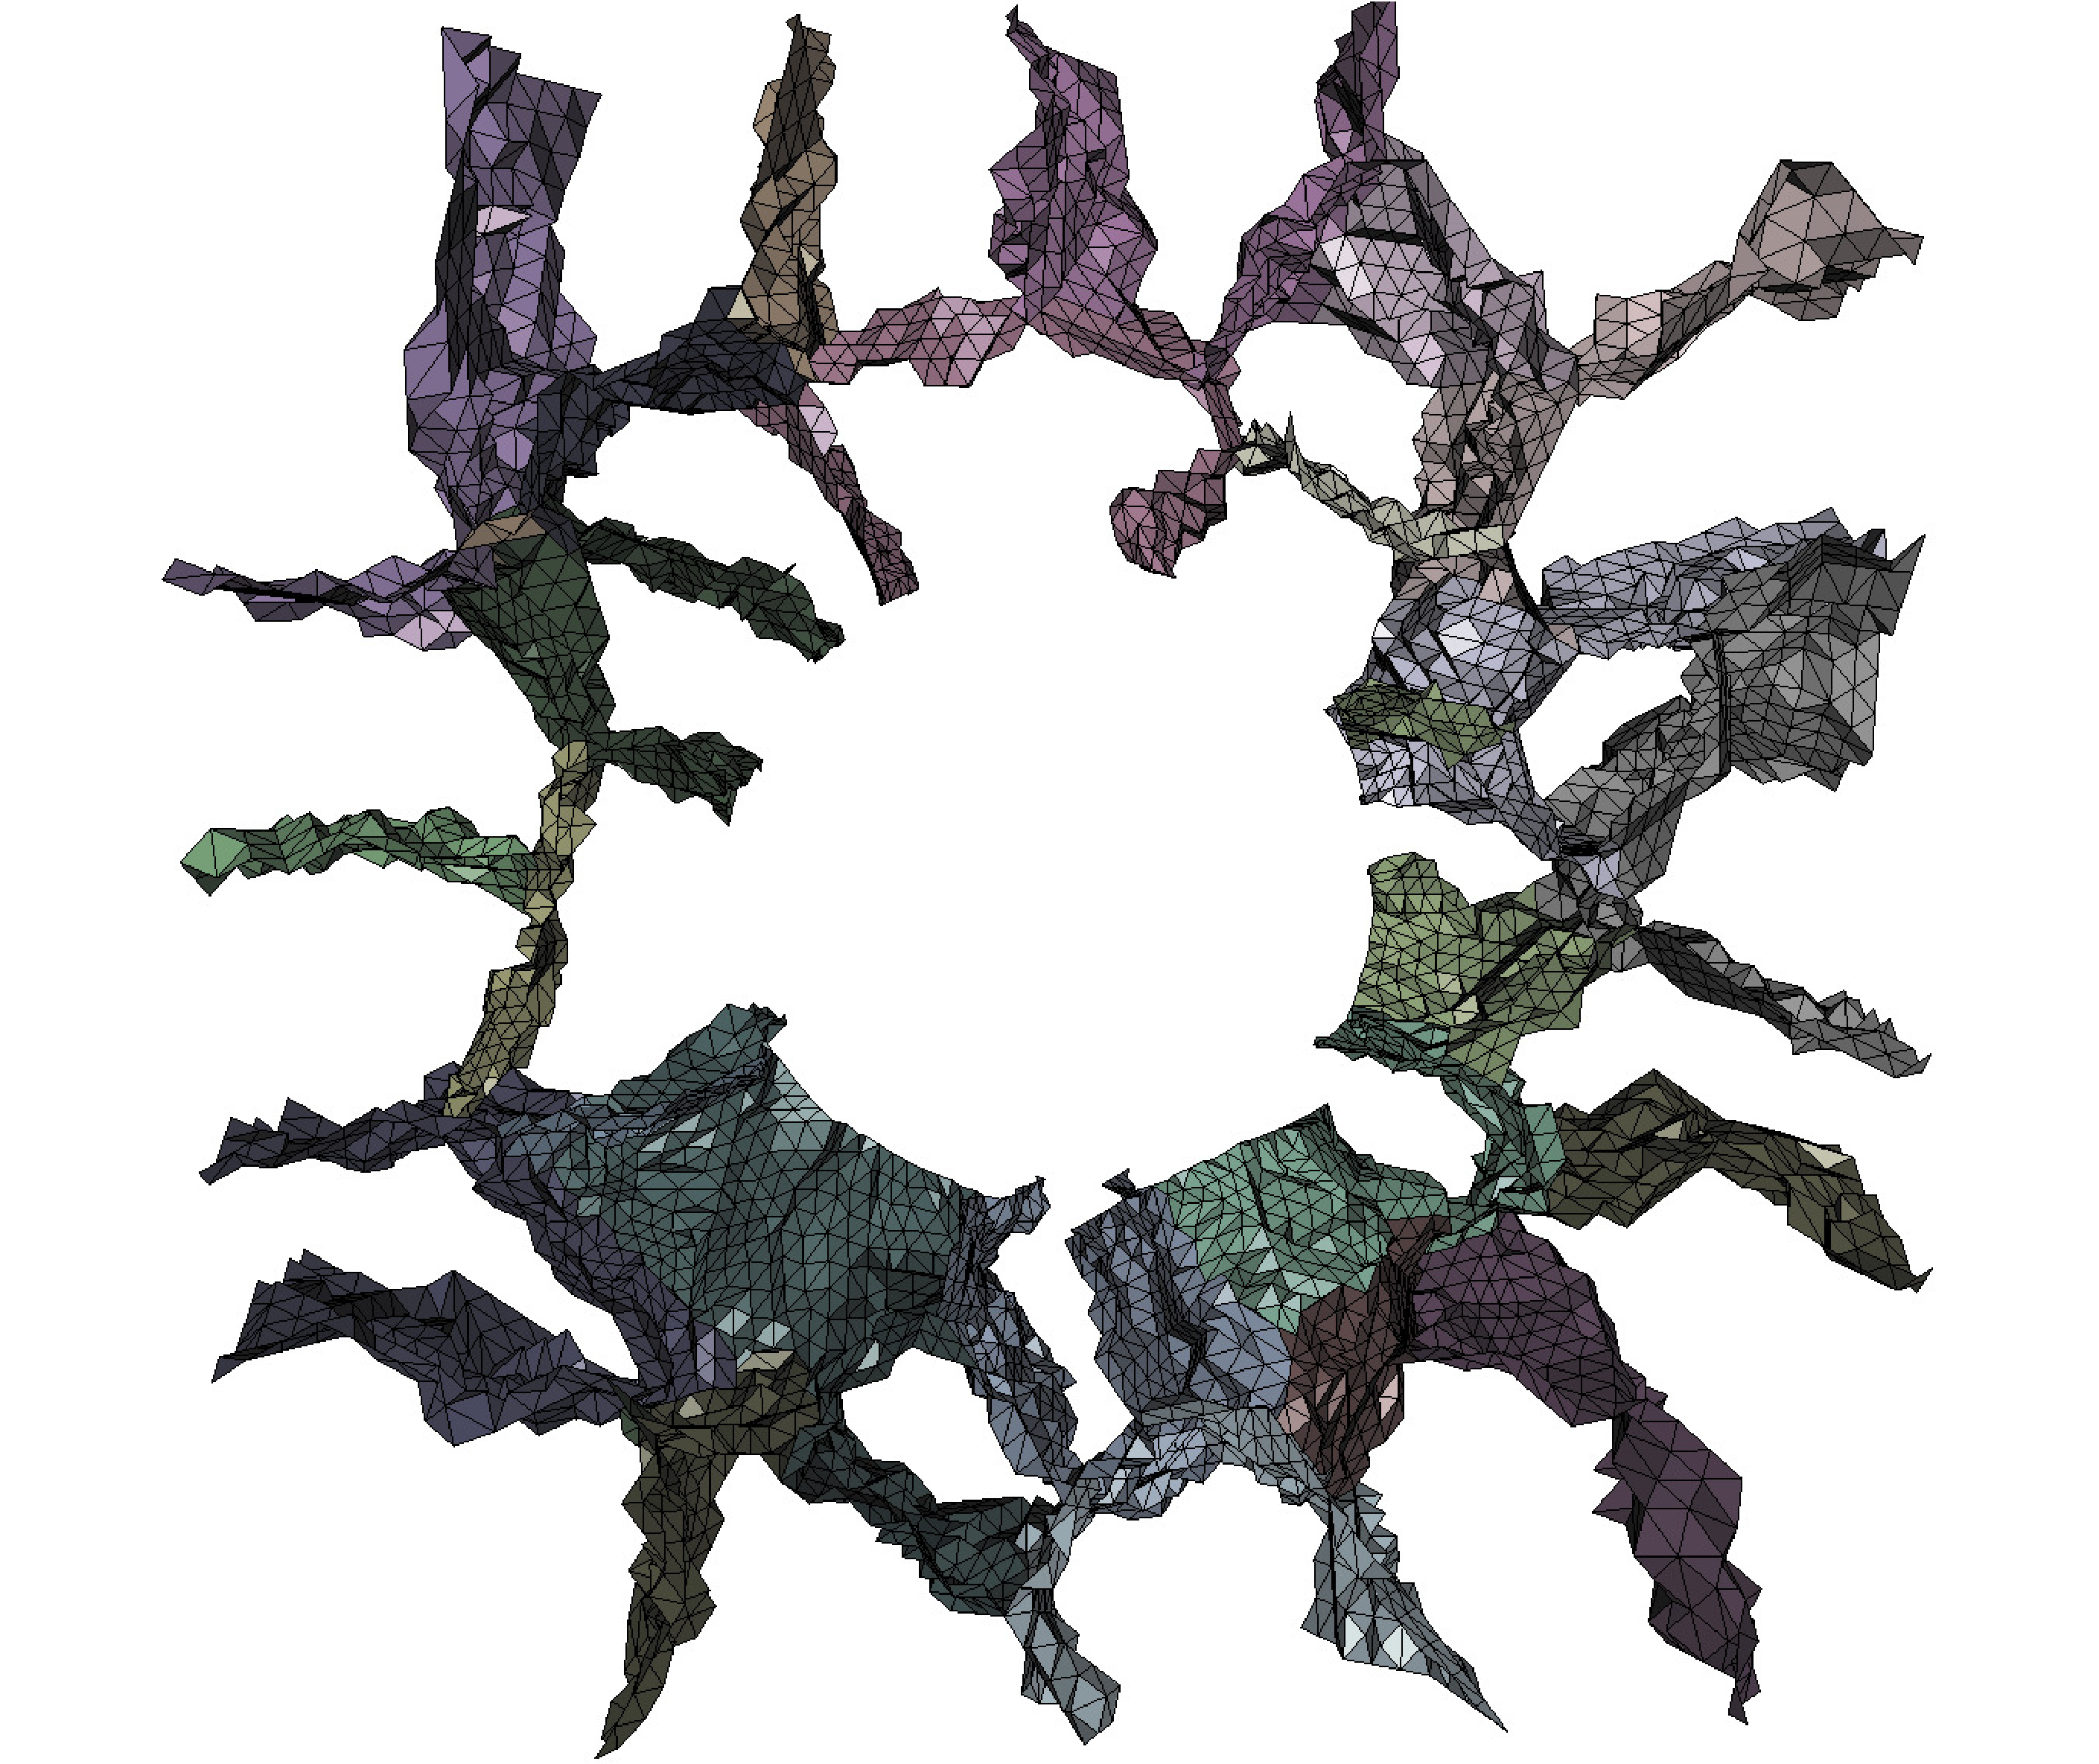
\includegraphics[width=2.3cm]{images/eps/rechteckring58534p_copy_entsaettigt3003.pdf}};

			\draw [arrow] (one) -- node[anchor=south] {\bf Linearize} (two);
			\draw [arrow] (two) -- node[anchor=south] {\bf Decompose} (three);
			\draw [arrow] (three) -- node[anchor=south] {\bf Build prec.} (four);
		\end{tikzpicture}
	\end{block}
	\begin{block}{\normalsize Nonlinear DD approach}
		\begin{tikzpicture}[node distance=2cm]
			% \node[inner sep=0pt] (one) at (-4.4,1.5){\Large\emph{\underline{Nonlinear DD approach}}};
			\node[inner sep=0pt] (one) at (-5,0)
			{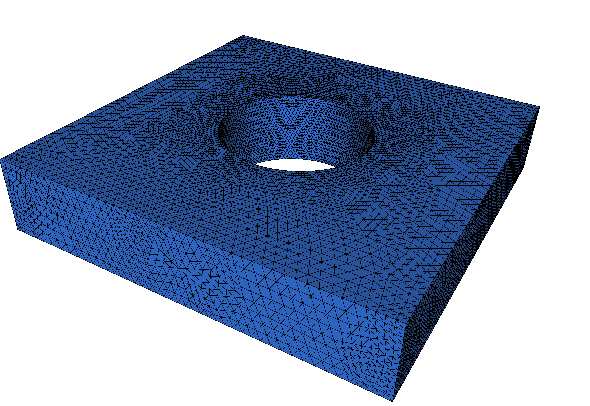
\includegraphics[width=2.9cm]{images/eps/rechteckring58534p_64001.pdf}};

			\node[inner sep=0pt] (two) at (-1,0)
			{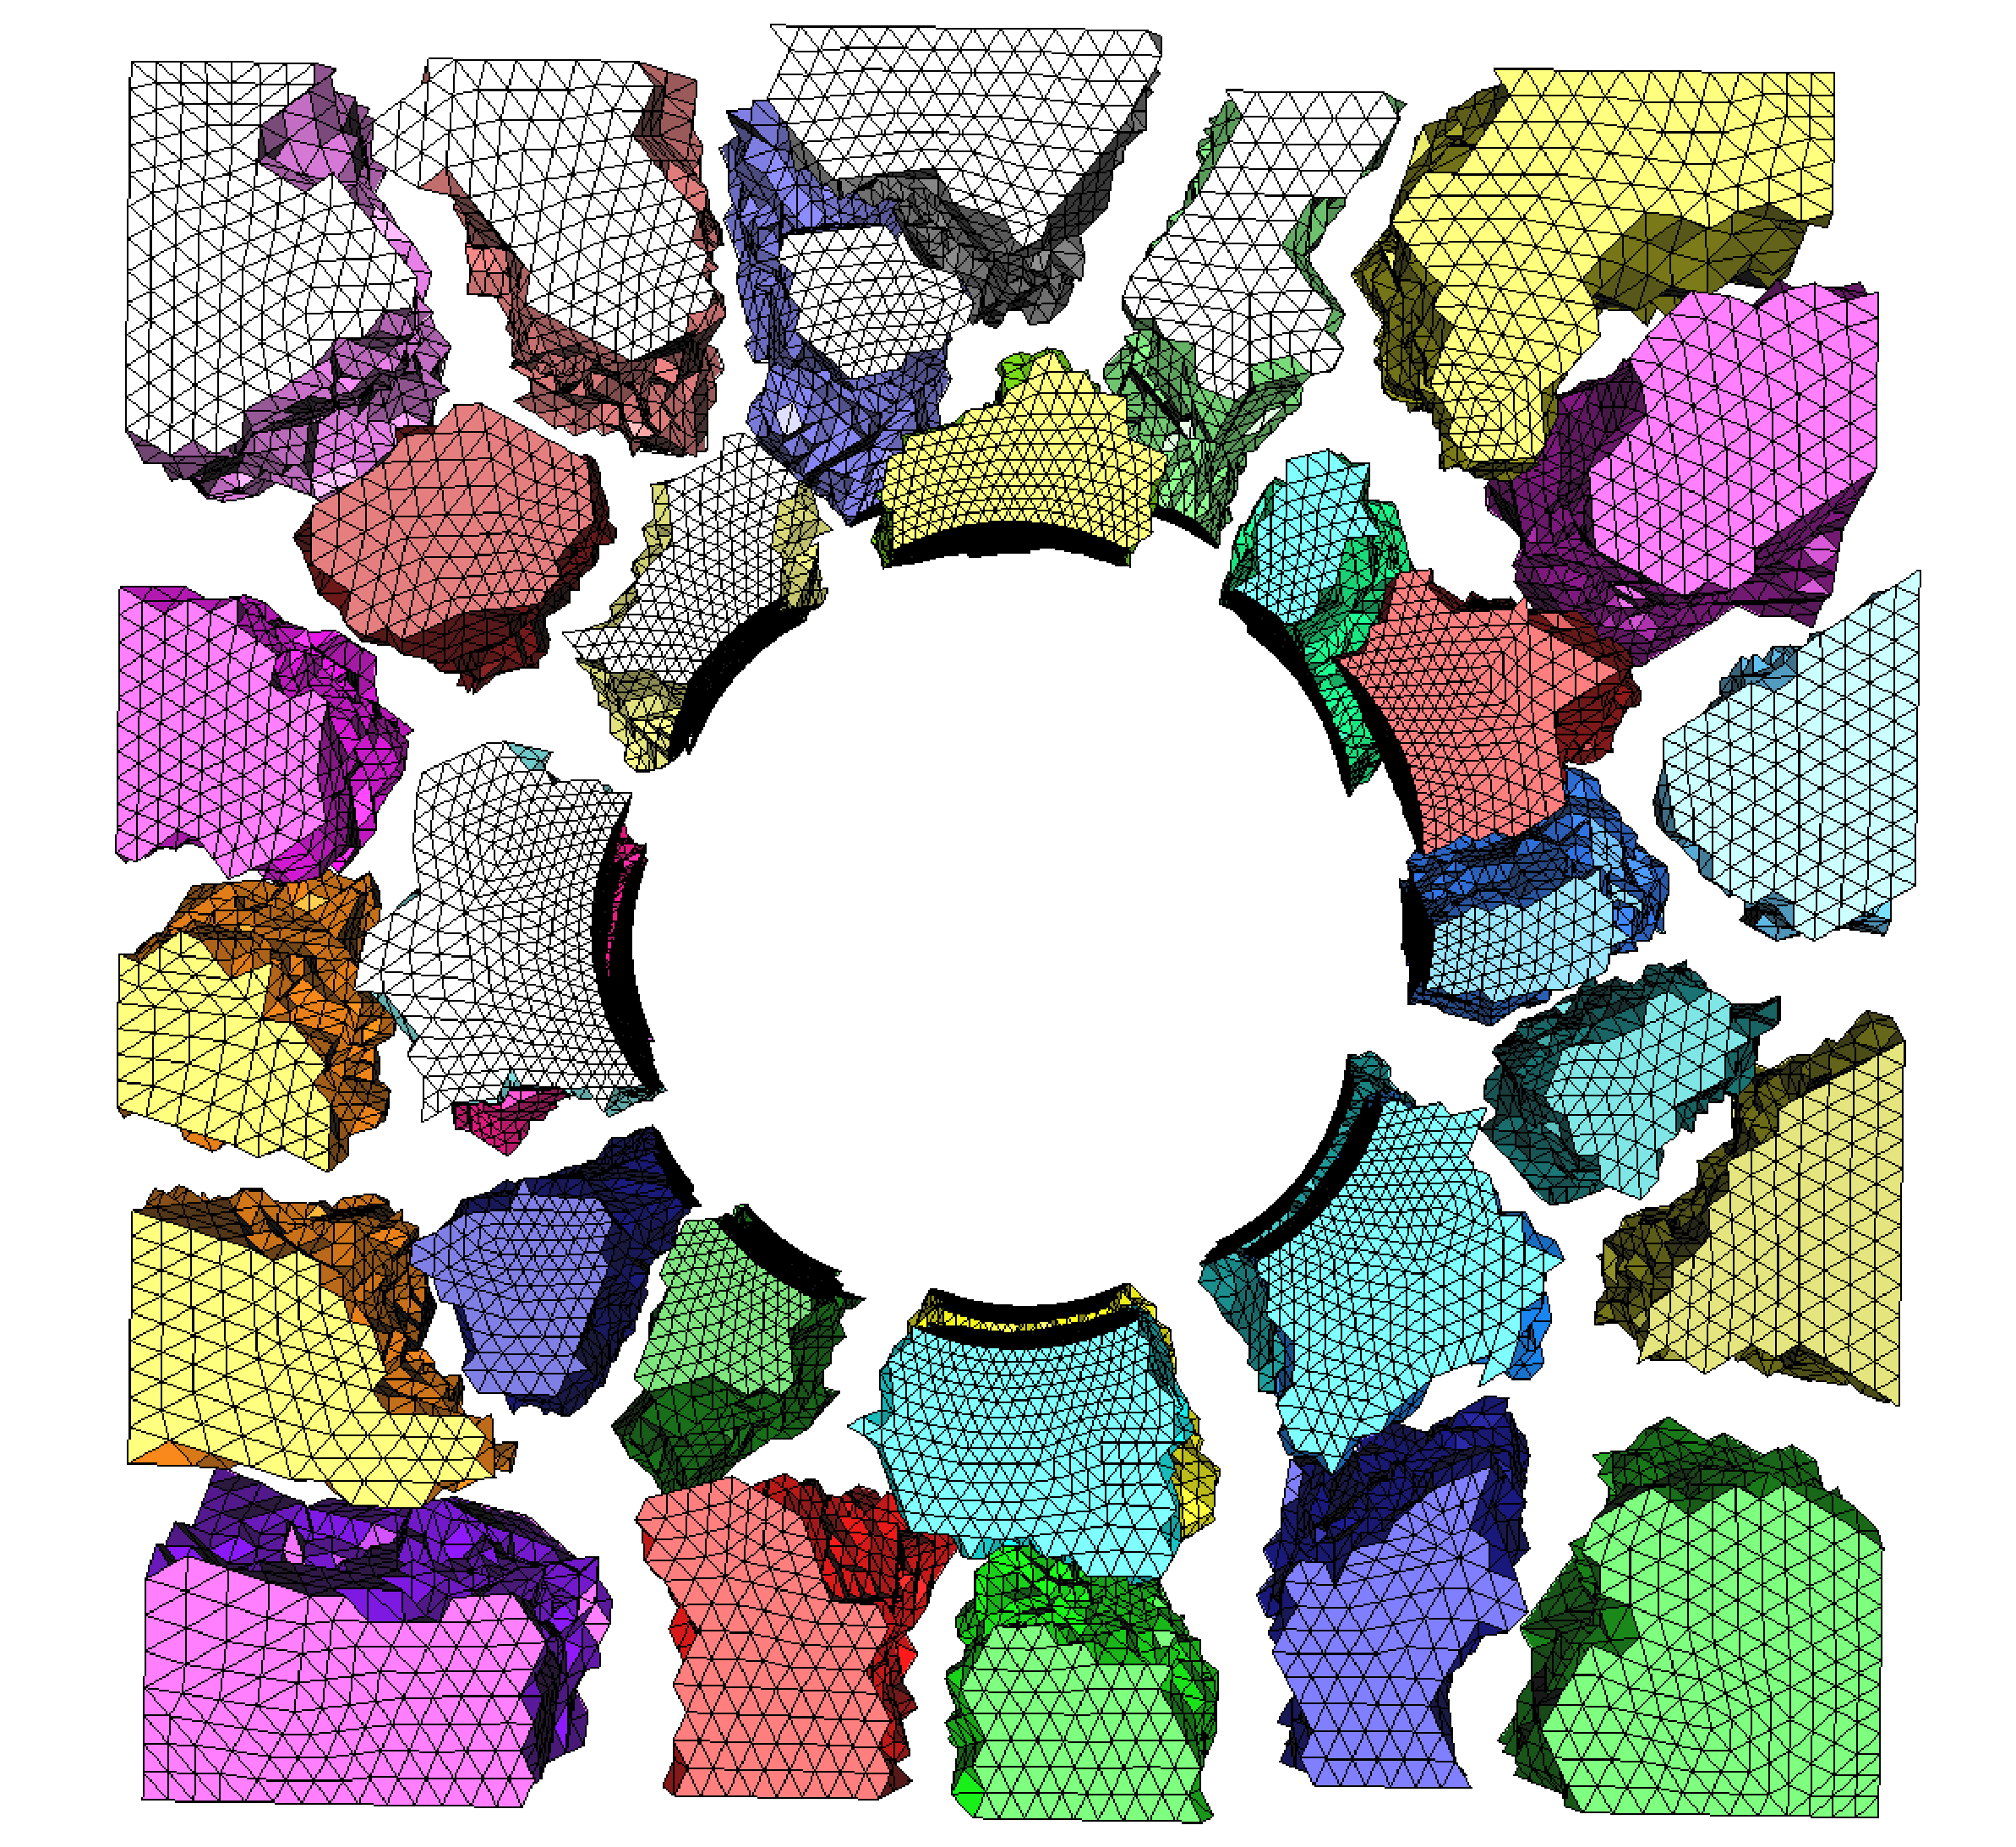
\includegraphics[width=2.0cm]{images/eps/exploded_5004.pdf}};
			\node[inner sep=0pt] (three) at (2.7,0)
			{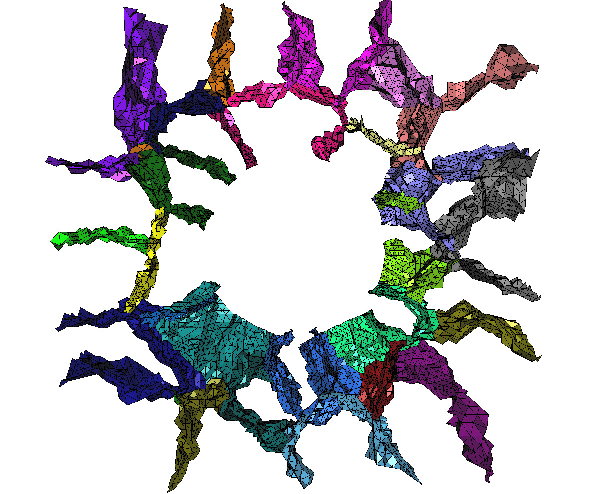
\includegraphics[width=2.3cm]{images/eps/rechteckring58534p_copy003.pdf}};
			\node[inner sep=0pt] (four) at (6,0)
			{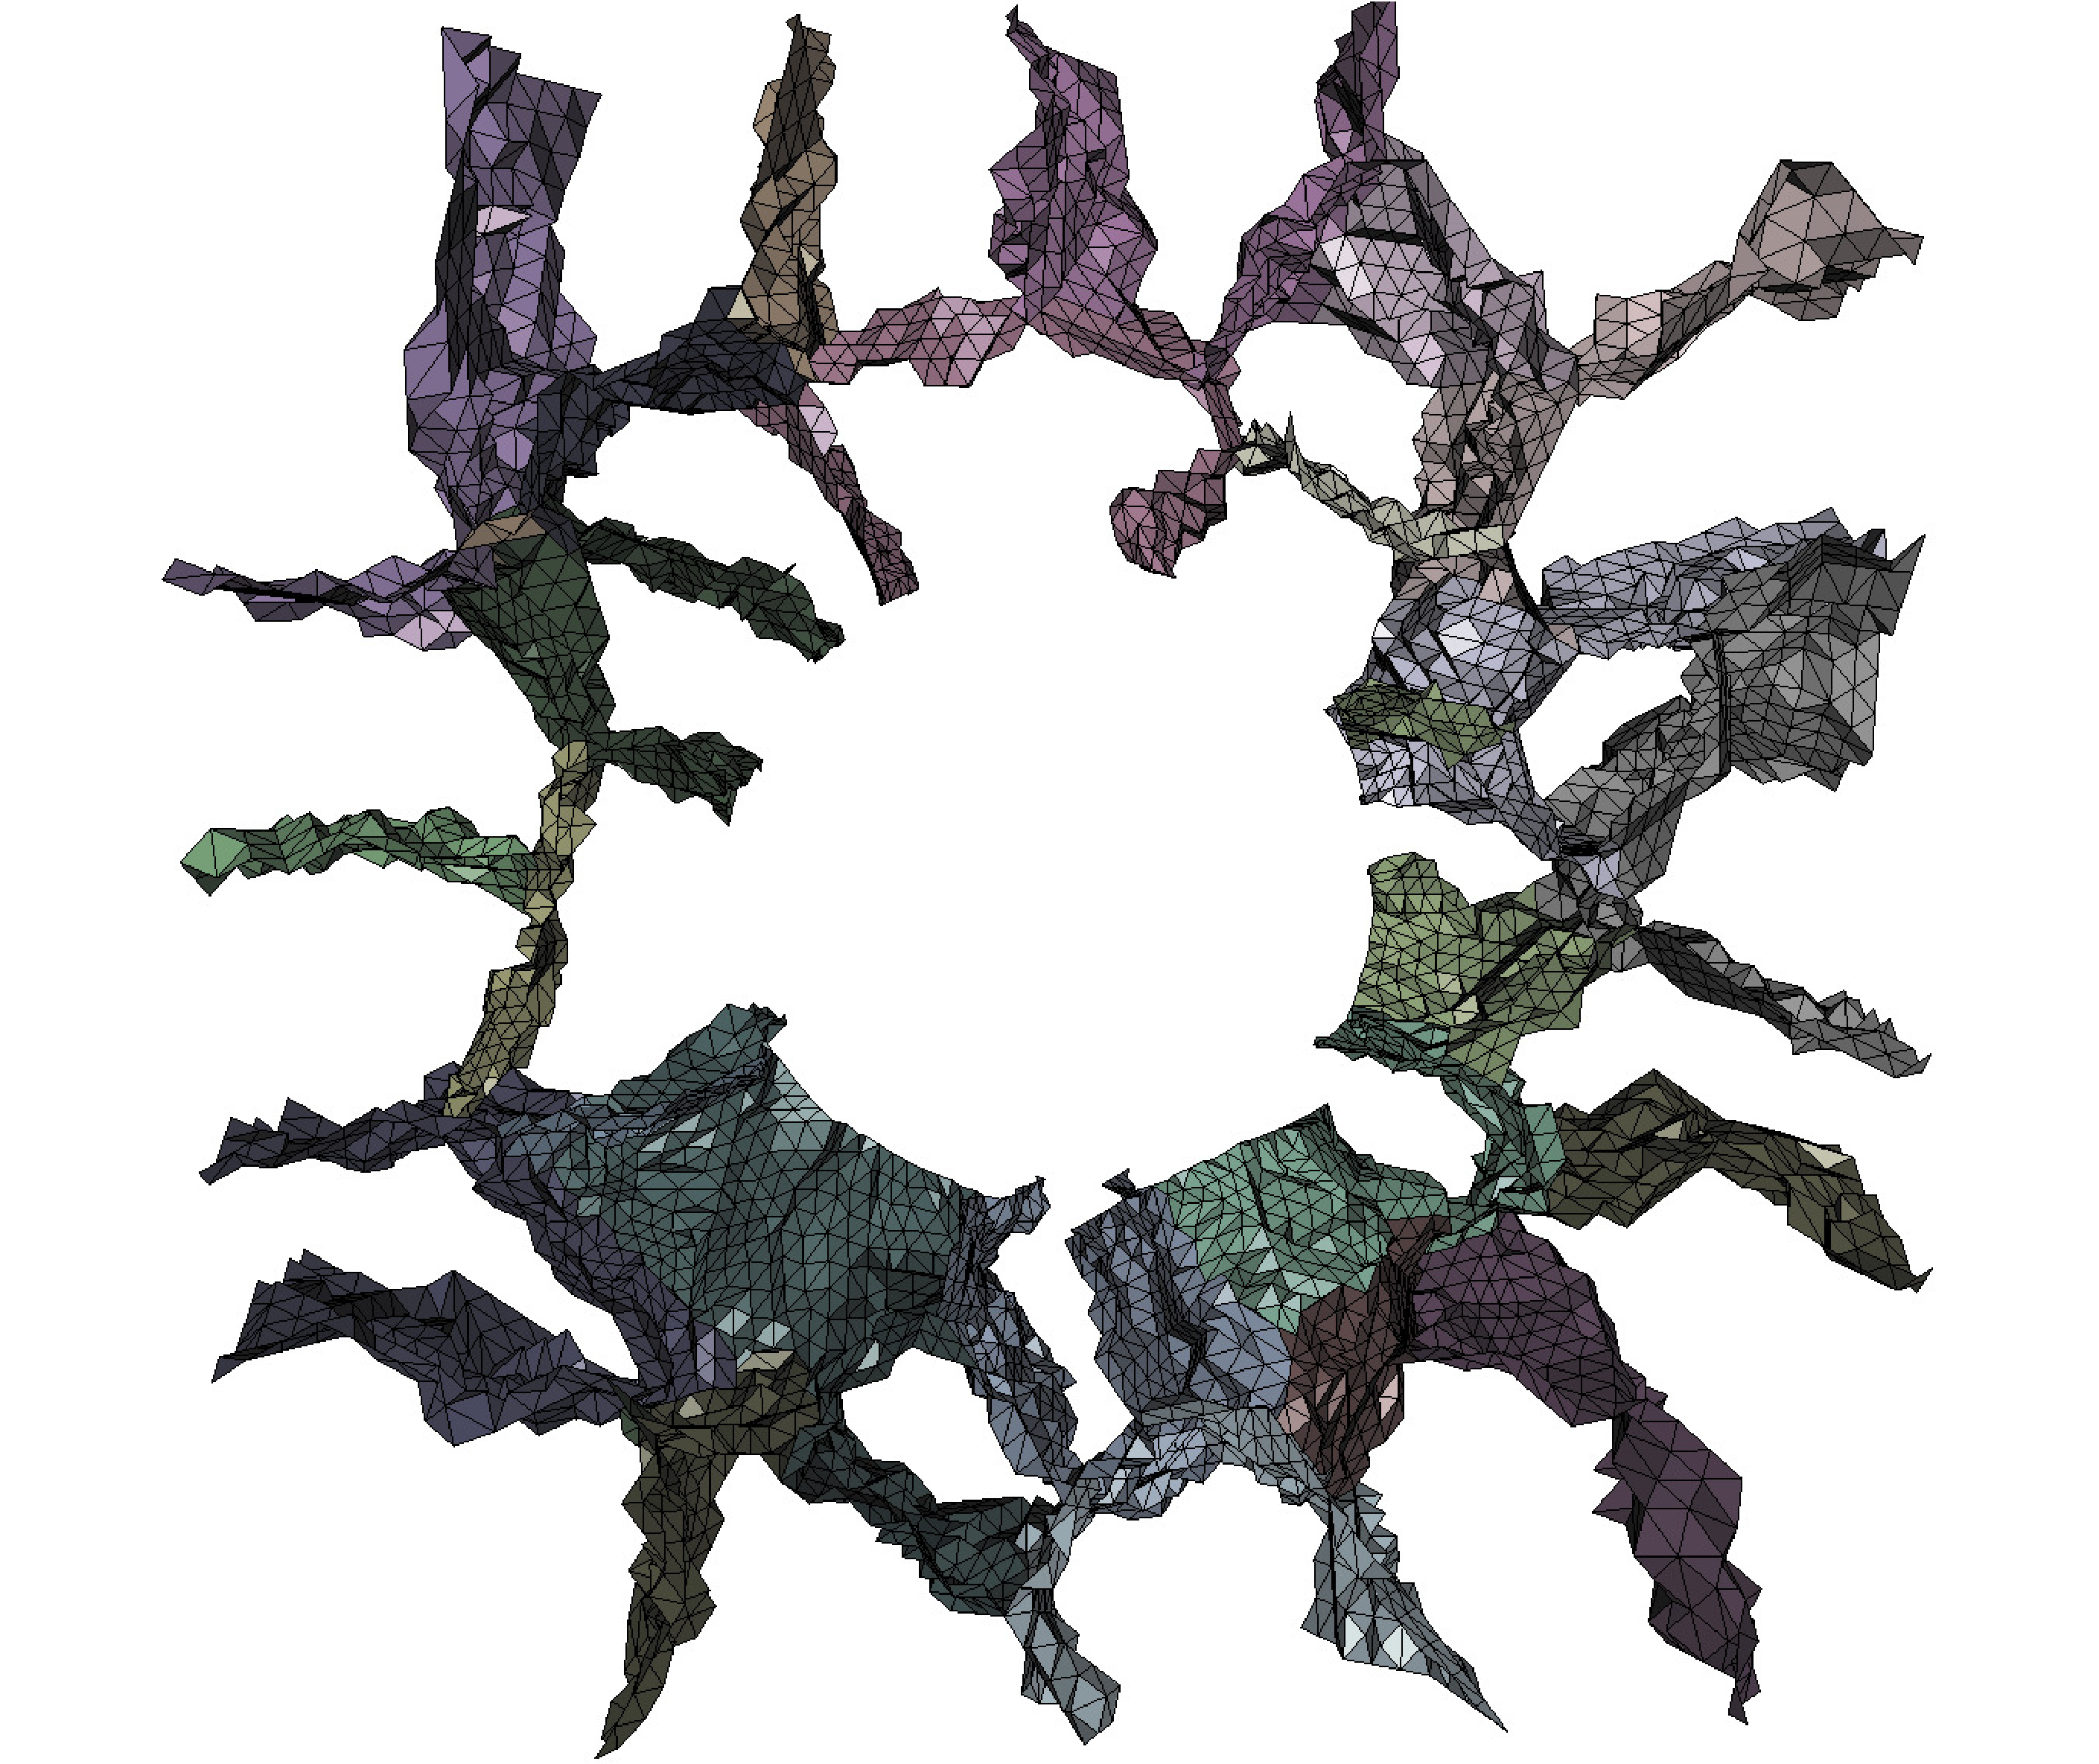
\includegraphics[width=2.3cm]{images/eps/rechteckring58534p_copy_entsaettigt3003.pdf}};


			\draw [arrow] (one) -- node[anchor=south] {\bf Decompose} (two);
			\draw [arrow, align=center, text width=2.3cm] (two) -- node[anchor=south] {\bf Build \mbox{alternative} problem} (three);
			\draw [arrow] (three) -- node[anchor=south] {\bf Linearize} (four);
		\end{tikzpicture}
	\end{block}
\end{frame}

\begin{frame}{Some References on Nonlinear Domain Decomposition Methods}
	\tiny
	\textbf{Nonlinear FETI-DP and Nonlinear BDDC:}\\
	Klawonn, Lanser, Rheinbach (2012, 2013, 2014, 2015, 2016, 2018), Klawonn, Lanser, Rheinbach, Uran (2017, 2018), Klawonn Lanser, Uran (2021, 2023), \dots\\~\\

	\textbf{Nonlinear Elimination:}\\
	Hwang, Lin, Cai (2010); Cai, Li (2011); Wang, Su, Cai (2015); Hwang, Su, Cai (2016); Gong, Cai (2018); Luo, Shiu, Chen, Cai (2019); Gong, Cai (2019); Liu, Hwang, Luo, Cai, Keyes (2022), \dots\\~\\

	\textbf{ASPIN:}\\
	Cai, Keyes 2002; Cai, Keyes, Marcinkowski 2002; Hwang, Cai 2005, 2007; Groß, Krause (2010, 2013), \dots\\~\\

	\textbf{MSPIN and Field-split methods:}\\
	Keyes, Liu, (2015, 2016,2021); Liu, Wei, Keyes (2017); Kopanicáková, Kothari, Krause (2023), \dots\\~\\

	\textbf{RASPEN:}\\
	Dolean, Gander, Kherijii, Kwok, Masson (2016)\\~\\

	\textbf{Nonlinear 2-Level Schwarz:}\\
	Heinlein, Lanser (2020); Heinlein, Klawonn, Lanser (2022)\\~\\

	\textbf{Nonlinear Neumann-Neumann:}\\ Bordeu, Boucard, Gosselet 2009\\~\\

	\textbf{Nonlinear FETI-1:}\\
	Pebrel, Rey, Gosselet 2008; Negrello, Gosselet, Rey (2021)\\~\\

	\textbf{Other DD work reversing linearization and decomposition:}\\
	Ganis, Juntunen, Pencheva, Wheeler, Yotov 2014; Ganis, Kumar, Pencheva, Wheeler, Yotov 2014
\end{frame}

% \begin{frame}{Motivation: linear vs nonlinear preconditioning}
% 	Discretized nonlinear partial differential equation: $F(u) = 0$
% 	\begin{columns}
% 		\begin{column}{0.5\textwidth}
% 			\vspace*{-4mm}
% 			\begin{block}{\normalsize Linear preconditioner}
% 				\begin{enumerate}
% 					\item Linearize:
% 					      \begin{equation*}
% 						      DF(u^k)\delta^{k+1} = F(u^k)
% 					      \end{equation*}
%                       \item Improve linear solver performance with e.g. linear-left preconditioner $\mathcal{M}$:
% 					      \begin{equation*}
% 						      \mathcal{M}^{-1}DF(u^k)\delta^{k+1} = \mathcal{M}^{-1}F(u^k)
% 					      \end{equation*}
% 				\end{enumerate}
% 				\vspace*{4mm}
% 				Goal:
% 				\begin{itemize}
% 					\item $\kappa(\mathcal{M}^{-1}DF(u^k)) \approx 1$
% 				\end{itemize}
% 			\end{block}
% 		\end{column}
% 		\begin{column}{0.5\textwidth}
% 			\vspace*{-4mm}
% 			\begin{block}{\normalsize Nonlinear preconditioner}
% 				\begin{enumerate}
% 					\item Reformulate the original nonlinear problem based on local nonlinear corrections
% 					      \begin{equation}
% 						      \mathcal{F}(u) = G(F(u)) = 0
% 					      \end{equation}
% 					\item Linearize $\mathcal{F}(u) = 0$ and solve iterativily
% 				\end{enumerate}
% 				Goal:
% 				\begin{itemize}
% 					\item $\mathcal{F}(u)$ more linear than $F(u)$
% 					\item $\mathcal{F}(u^*) = 0 \iff F(u^*) = 0$
% 				\end{itemize}
% 			\end{block}
% 		\end{column}
% 	\end{columns}
% \end{frame}

\begin{frame}{One-level nonlinear Schwarz \footnote{\tiny Cai and Keyes 2002}}%: Nonlinearly preconditioned inexact Newton algorithms}}
	% \only<1-3>{
	Discretized nonlinear partial differential equation: $F(u) = 0$
	\vspace*{-5mm}
	% }
	% \only<4->{
	%     \vspace*{-10mm}
	% }

	\begin{columns}
		\begin{column}{0.47\textwidth}
			\begin{block}<1->{\normalsize Nonlinear corrections $T_i(u): V\mapsto V_i$}
				\vspace*{-5mm}
				\begin{align*}
					 & R_iF(u-P_iT_i(u))  = 0, \quad i = 1,2,\dots,N                \\
					 & \text{with}\quad R_i:V\mapsto V_i\text{,}\, P_i:V_i\mapsto V
				\end{align*}
			\end{block}
		\end{column}
        \hspace{-3mm}
		\begin{column}{0.47\textwidth}
			\begin{block}<2->{\normalsize Define an alternative nonlinear problem}
				\begin{equation*}
					\mathcal{F}_1(u) \coloneqq \sum_{i=1}^N\alert<4>{P_iT_i(u)} = 0
				\end{equation*}
			\end{block}
		\end{column}
	\end{columns}
	% \begin{columns}
	% 	\begin{column}{1.02\textwidth}
			\begin{block}<3->{\normalsize Nonlinear Schwarz method results by solving $\mathcal{F}_1(u) = 0$ with Newton's method.\newline Setting $u_i = u-P_iT_i(u)$ the Jacobian can be formulated as:}
				\vspace*{-2mm}
				\begin{align*}
					D\mathcal{F}_1(u^k)  = \sum_{i = 1}^NP_iDT_i(u^k) = \sum_{i=1}^N\alert<4>{P_i(R_iDF(u_i^k)P_i)^{-1}R_iDF(u_i^k)}
				\end{align*}
			\end{block}
	% 	\end{column}
	% \end{columns}

	\only<4>{%
		\tikz[overlay,remember picture]
		\node[fill=white,text=red] at ([xshift=0cm,yshift=-3cm]current page.center){\Large Parallel execution!};
	}
	% \only<4>{%
	% \begin{itemize}
	% 	\item For the one-level nonlinear Schwarz method the solutions of $F(u) = 0$ and $\mathcal{F}_1(u) = 0$ are equivalent
	% 	\item The global operators $DF(u_i)$ only need to be assembled locally
	% \end{itemize}
	% }
\end{frame}

\begin{frame}{Two-level additive nonlinear Schwarz \footnote{\tiny Heinlein, Lanser (2020)} \footnote{\tiny Heinlein, Lanser, Klawonn (2022)}}
	% \vspace*{-5mm}
	\begin{columns}
		\begin{column}{0.47\textwidth}
			\begin{block}{\normalsize Nonlinear corrections $T_i(u)$}
				\vspace*{-4mm}
				\begin{align*}
					 & R_iF(u-P_iT_i(u))  = 0, \quad i = \alert{0},1,\dots,N      \\
					 & \text{with}\quad R_i:V\mapsto V_i\text{,}\, P_i:V_i\mapsto V
				\end{align*}
			\end{block}
		\end{column}
        \hspace{-3mm}
		\begin{column}{0.47\textwidth}
			\begin{block}{\normalsize Alternative nonlinear problem}
				\vspace*{-4mm}
				\begin{equation*}
					\mathcal{F}_A(u) \coloneqq \alert{P_0T_0(u)} + \sum_{i=1}^NP_iT_i(u) = 0
				\end{equation*}
			\end{block}
		\end{column}
	\end{columns}
	\begin{block}{\normalsize The Jacobian}
		\vspace*{-2mm}
		\begin{align*}
			D\mathcal{F}_A(u^k)  = \alert{P_0(R_0DF(u_0^k)P_0)^{-1}R_0DF(u_0^k)} + \sum_{i=1}^NP_i(R_iDF(u_i^k)P_i)^{-1}R_iDF(u_i^k)
		\end{align*}
	\end{block}
\end{frame}

\begin{frame}{Two-level hybrid nonlinear Schwarz  \footnote[2]{\tiny Heinlein, Lanser (2020)} \footnote[3]{\tiny Heinlein, Lanser, Klawonn (2022)}}
	\vspace*{-5mm}
	\begin{block}{\normalsize Alternative nonlinear problem}
		\begin{equation*}
			\mathcal{F}_{hybrid}(u) \coloneqq \sum_{i=1}^NP_iT_i(u-P_0T_0(u)) + P_0T_0(u),
		\end{equation*}
	\end{block}
	\begin{block}{\normalsize The Jacobian}
		\vspace*{-2mm}
		\begin{equation*}
			D\mathcal{F}_{hybrid}(u^k) = I - \left(I-\sum_{i=1}^NQ_i(v_i)\right)(I-Q_0(u_0))
		\end{equation*}
		\begin{align*}
			\text{with}\quad Q_i(u) & \coloneqq P_i(R_iDF(u)P_i)^{-1}R_iDF(u), \\
			u_i                     & \coloneqq u-P_iT_i(u)                    \\
			\text{and}\quad v_i     & \coloneqq u_0-P_iT_i(u_0)
		\end{align*}
	\end{block}
\end{frame}

\begin{frame}{Two-level nonlinear Schwarz}%: Nonlinearly preconditioned inexact Newton algorithms}}
	\begin{tikzpicture}[transform shape]
    % Define coordinates for the main elements
    \coordinate (leftImg) at (0,0);
    \coordinate (topImg) at (5,2.5);
    \coordinate (bottomImg) at (5,-2.5);
    \coordinate (rightEq) at (10,1.0);
    
    % Place the placeholder images (blue rectangles with numerical solution)
    \node[inner sep=0] (leftRectangle) at (leftImg) 
        {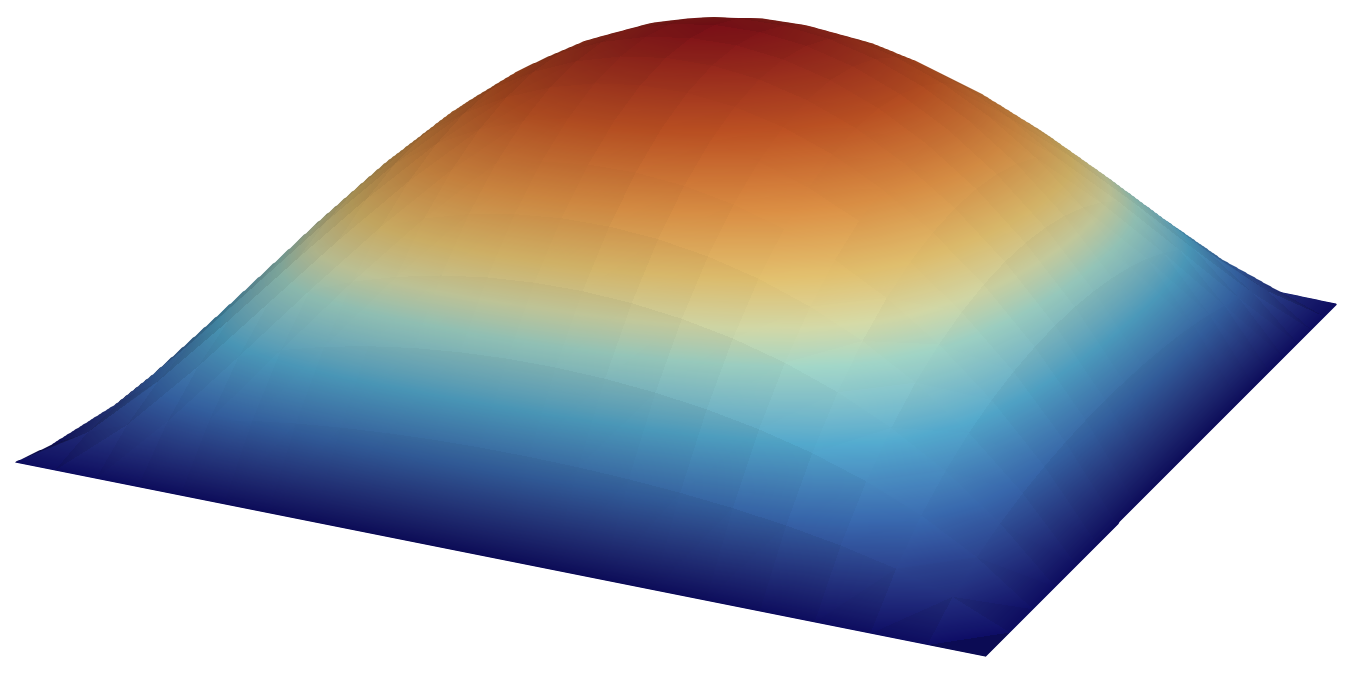
\includegraphics[width=5cm]{images/global-solution.png}};
    \node[inner sep=0] (topRectangle) at (topImg) 
        {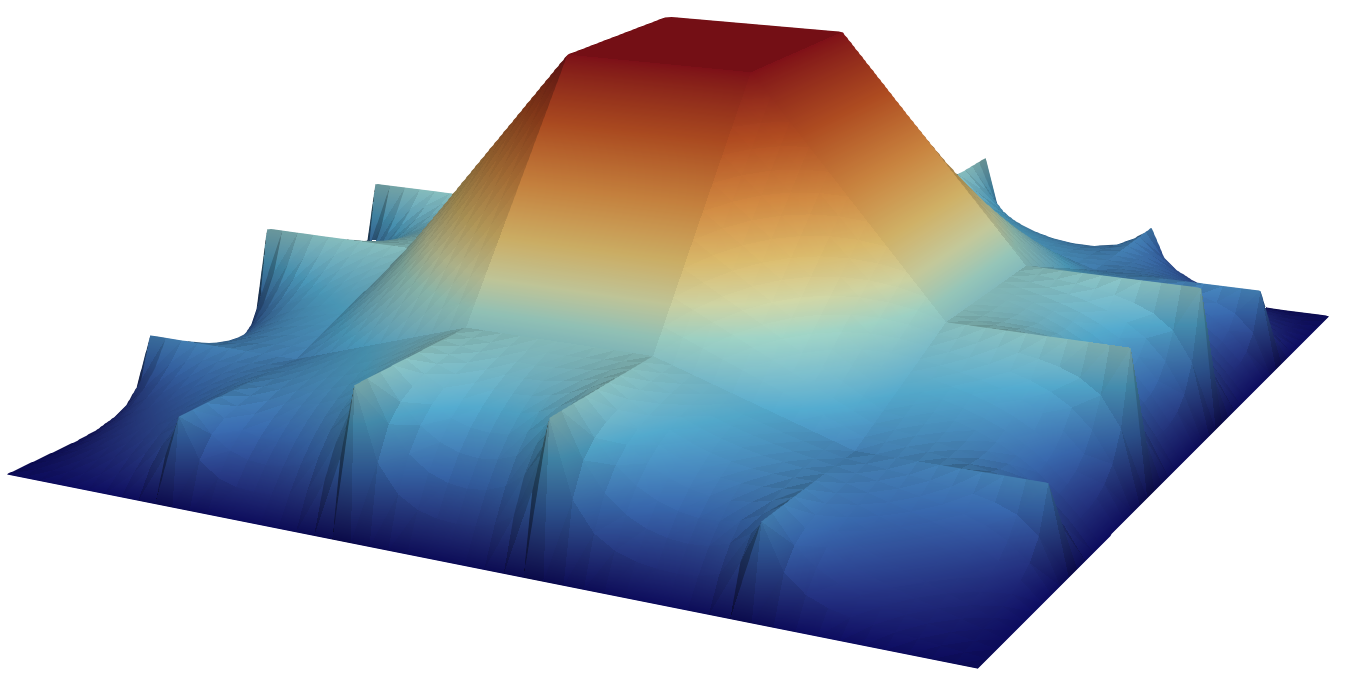
\includegraphics[width=5cm]{images/coarse-solution.png}};
     \node[inner sep=0] (bottomRectangle) at (bottomImg) 
        {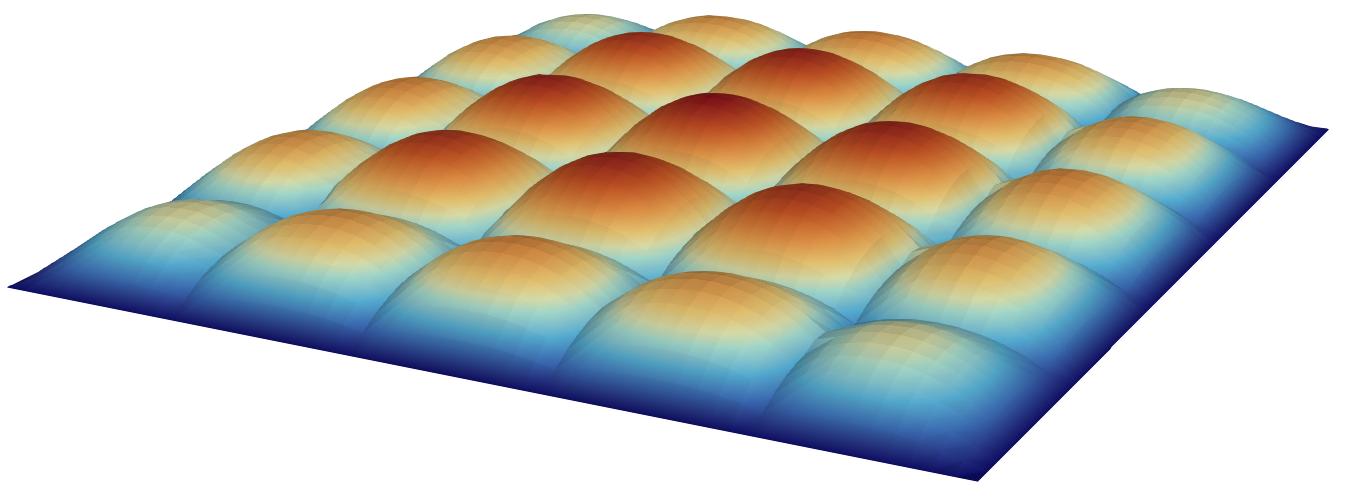
\includegraphics[width=5cm]{images/local-solutions.png}};
    
    \node[fill=white, fill opacity=0.7, text opacity=1, yshift=5mm, xshift=2mm, text width = 35mm] at (leftRectangle.north) {\small Discretized nonlinear problem};
    \node[yshift=0cm, fill=white, fill opacity=0.9, text opacity=1] at (leftRectangle.south) {\small $F(u) = 0$};

    \node[yshift=0cm, fill=white, fill opacity=0.9, text opacity=1] at (bottomRectangle.south) {\small $R_i F\left(\bm{u} - R_i^T T_i(\bm{u})\right) = 0$};
    
    \node [fill=white, fill opacity=0.9, text opacity=1] at (topRectangle.south){\small $\Phi^T F\left(\bm{u} - \Phi T_0(\bm{u})\right) = 0$};
    
    \node[align=left, fill=white, fill opacity=0.7, text opacity=1, text width = 4.5cm] at (9.6,-1.3){\small Solve with Newton's method for nonlinear corrections $T_i(u), \quad i = 0,\ldots, N$};
    
    \node[draw, rectangle, minimum width=4cm, minimum height=1cm] (boxedEq) at (rightEq) {\small $\mathcal{F}(\bm{u}) = \sum_{i=0}^{N} R_i^T T_i(\bm{u})$};
    
    % Arrows
    \draw[-{Stealth[length=3mm, width=2mm]}] ($(leftRectangle.north east) + (-0.5, -0.5)$) -- ($(topRectangle.south west) + (0.3, 0.3)$);
    \draw[-{Stealth[length=3mm, width=2mm]}] ($(leftRectangle.south east) + (-0.7, 0.4)$) -- ($(bottomRectangle.north west) + (0.8, -0.2)$);
    \draw[-{Stealth[length=3mm, width=2mm]}] ($(topRectangle.south east)+ (-0.3, 0.7)$) -- ($(boxedEq.north west)+ (-0.1, 0.1)$);
    \draw[-{Stealth[length=3mm, width=2mm]}] ($(bottomRectangle.north east)+ (-0.8, -0.1)$) -- ($(boxedEq.south west)+ (-0.1, -0.1)$);
\end{tikzpicture}

\end{frame}
